\documentclass[border=0.2cm]{standalone}

%\renewcommand{\raggedsection}{\centering}
\usepackage{sectsty}
\usepackage{lipsum}
\usepackage{cases}
\usepackage{tikz}
\usetikzlibrary{shapes.geometric}
\usetikzlibrary{calc}
\usetikzlibrary{arrows}
\usetikzlibrary{decorations.pathreplacing}
\usetikzlibrary{arrows.meta}

\begin{document}
	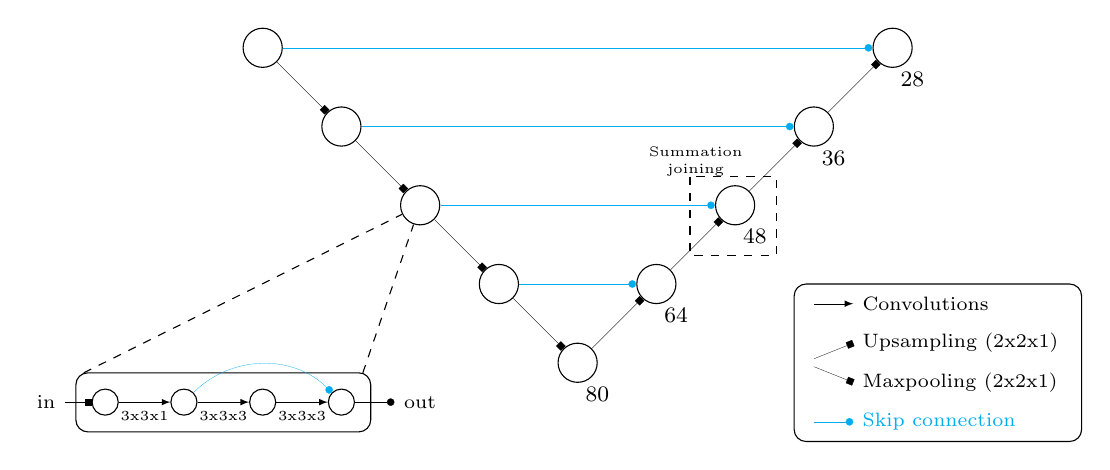
\begin{tikzpicture}
		\node[circle,draw, scale=1.5] (n1) at (-4,4) {};
		\node[circle,draw, scale=1.5] (n2) at (-3,3) {};
		\node[circle,draw, scale=1.5] (n3) at (-2,2) {};
		\node[circle,draw, scale=1.5] (n4) at (-1,1) {};

		\node[circle,draw, scale=1.5] (n5) at (0,0) {};
		\node (n51) at (0.25,-0.4) {\footnotesize $80$};

		\node[circle,draw, scale=1.5] (n6) at (1,1) {};
		\node (n61) at (1.25,0.6) {\footnotesize $64$};
		\node[circle,draw, scale=1.5] (n7) at (2,2) {};
		\node (n71) at (2.25,1.6) {\footnotesize $48$};
		\draw [dashed] ($(n71.north west)+(-0.55, 0.55)$) rectangle ($(n71.north east)+(0,-0.45)$);
		\node (n71text) at (1.5,2.55) {\tiny \begin{tabular}{c} Summation \\ joining \end{tabular}};
		\node[circle,draw, scale=1.5] (n8) at (3,3) {};
		\node (n81) at (3.25,2.6) {\footnotesize $36$};
		\node[circle,draw, scale=1.5] (n9) at (4,4) {};
		\node (n91) at (4.25,3.6) {\footnotesize $28$};
		
		% Connections
		\draw [-{Square}, line width=0.1pt] (n1) edge (n2);
		\draw [-{Square}, line width=0.1pt] (n2) edge (n3);
		\draw [-{Square}, line width=0.1pt] (n3) edge (n4);
		\draw [-{Square}, line width=0.1pt] (n4) edge (n5);
		
		\draw [-{Square}, line width=0.1pt] (n5) edge (n6);
		\draw [-{Square}, line width=0.1pt] (n6) edge (n7);
		\draw [-{Square}, line width=0.1pt] (n7) edge (n8);
		\draw [-{Square}, line width=0.1pt] (n8) edge (n9);

		\draw [-{Circle}, line width=0.1pt, cyan] (n1) edge (n9);
		\draw [-{Circle}, line width=0.1pt, cyan] (n2) edge (n8);
		\draw [-{Circle}, line width=0.1pt, cyan] (n3) edge (n7);
		\draw [-{Circle}, line width=0.1pt, cyan] (n4) edge (n6);

		% Residual module
		\node (in_res) at (-6.75,-0.5) {\scriptsize in};
		\node[circle,draw] (res1) at (-6,-0.5) {};
		\node[circle,draw] (res2) at (-5,-0.5) {};
		\node[circle,draw] (res3) at (-4,-0.5) {};
		\node[circle,draw] (res4) at (-3,-0.5) {};
		\node (out_res) at (-2,-0.5) {\scriptsize out};
		\draw[rounded corners=1ex] ($(res1.north west)+(-0.25, 0.25)$) rectangle ($(res4.north east)+(0.25,-0.5)$);

		\path [->, -latex, line width=0.1pt] (res1) edge node [below] {\tiny 3x3x1} (res2);
		\path [->, -latex, line width=0.1pt] (res2) edge node [below] {\tiny 3x3x3} (res3);
		\path [->, -latex, line width=0.1pt] (res3) edge node [below] {\tiny 3x3x3} (res4);
		\draw [-{Square}, line width=0.1pt] (in_res) edge (res1);
		\draw [-{Circle}, line width=0.1pt] (res4) edge (out_res);
		\path [dashed] ($(res1.north west)+(-0.15, 0.25)$) edge (n3);
		\path [dashed] ($(res4.north east)+(0.15,0.25)$) edge (n3);
		\path [-{Circle}, bend left=45, line width=0.1pt, cyan] (res2) edge (res4);

		%Description
		\draw[-latex, line width=0.1pt] (3,0.75)--(3.5,0.75) node[right] {\scriptsize Convolutions};
		\draw[-{Square}, line width=0.1pt] (3,0.05)--(3.5,0.25) node[right, text centered] {\scriptsize Upsampling (2x2x1)};
		\draw[-{Square}, line width=0.1pt] (3,-0.05)--(3.5,-0.25) node[right]{\scriptsize Maxpooling (2x2x1)};
		\draw[-{Circle}, line width=0.1pt, cyan] (3,-0.75)--(3.5,-0.75) node[right]{\scriptsize Skip connection};
		\draw[rounded corners=1ex] (2.75, 1) rectangle (6.4, -1);

		

	\end{tikzpicture}
\end{document}
